% In principle, this file can be redistributed and/or modified under
% the terms of the GNU Public License, version 2.
%
% However, this file is supposed to be a template to be modified
% for your own needs. For this reason, if you use this file as a
% template and not specifically distribute it as part of a another
% package/program, I grant the extra permission to freely copy and
% modify this file as you see fit and even to delete this copyright
% notice. 

\documentclass{beamer}

% There are many different themes available for Beamer. A comprehensive
% list with examples is given here:
% http://deic.uab.es/~iblanes/beamer_gallery/index_by_theme.html
% You can uncomment the themes below if you would like to use a different
% one:
%\usetheme{AnnArbor}
%\usetheme{Antibes}
%\usetheme{Bergen}
%\usetheme{Berkeley}
%\usetheme{Berlin}
%\usetheme{Boadilla}
%\usetheme{boxes}
%\usetheme{CambridgeUS}
%\usetheme{Copenhagen}
%\usetheme{Darmstadt}
%\usetheme{default}
%\usetheme{Frankfurt}
%\usetheme{Goettingen}
%\usetheme{Hannover}
%\usetheme{Ilmenau}
%\usetheme{JuanLesPins}
%\usetheme{Luebeck}
\usetheme{Madrid}
%\usetheme{Malmoe}
%\usetheme{Marburg}
%\usetheme{Montpellier}
%\usetheme{PaloAlto}
%\usetheme{Pittsburgh}
%\usetheme{Rochester}
%\usetheme{Singapore}
%\usetheme{Szeged}
%\usetheme{Warsaw}
\usepackage{textcomp}
\usepackage{graphicx}

\pgfdeclareimage[height=0.6cm]{university-logo}{iiitd-logo.png}


\title[TAPIR]{Tapir: Embedding Fork-Join Parallelism
into LLVM\textquotesingle s Intermediate Representation}

% A subtitle is optional and this may be deleted
\subtitle{January 2017 PPoPP '17}

\author{Pavas~Handa \and M. F. R.~Wani}
% - Give the names in the same order as the appear in the paper.
% - Use the \inst{?} command only if the authors have different
%   affiliation.

\institute[IIIT-D] % (optional, but mostly needed)
{
  Department of Computer Science \\
  IIIT-D
}
% - Use the \inst command only if there are several affiliations.
% - Keep it simple, no one is interested in your street address.

\date[CSE502 -- March 2017]{Class Presentation, March 2017}
% - Either use conference name or its abbreviation.
% - Not really informative to the audience, more for people (including
%   yourself) who are reading the slides online

\subject{Parallel Programming and Compilers}
\logo{\pgfuseimage{university-logo}}

% This is only inserted into the PDF information catalog. Can be left
% out. 

% If you have a file called "university-logo-filename.xxx", where xxx
% is a graphic format that can be processed by latex or pdflatex,
% resp., then you can add a logo as follows:

% \pgfdeclareimage[height=0.5cm]{university-logo}{university-logo-filename}
% \logo{\pgfuseimage{university-logo}}

% Delete this, if you do not want the table of contents to pop up at
% the beginning of each subsection:
\AtBeginSubsection[]
{
  \begin{frame}<beamer>{Outline}
    \tableofcontents[currentsection,currentsubsection]
  \end{frame}
}

% Let's get started
\begin{document}

\begin{frame}
  \titlepage
\end{frame}

\begin{frame}{Outline}
  \tableofcontents
  % You might wish to add the option [pausesections]
\end{frame}

% Section and subsections will appear in the presentation overview
% and table of contents.
\section{Foundations}

\subsection{Introduction}

\begin{frame}{LLVM: Low Level Virtual Machine}{Is it yet another compiler ? whatever... Why should I care ?}
\begin{columns}[T]
\begin{column}{0.5\textwidth}
  \begin{itemize}
  \item {
    Compiler Design 101:
    \begin{itemize}
    \item Lexer (\texttt{lex})
    \item Parser (\texttt{yacc})
    \item Semantic Analyser
    \item Intermediate Code
    \item IR Optimizer
    \item Target Code
    \item Target Code Optimizer
    \end{itemize}
  }
  \item {
    \texttt{LLVM} provides a \alert{tool-chain}.
  }
  \item {
    Most important is \alert{LLVM-IR}.
  }
  \item {
    \texttt{LLVM} is modular, unlike \texttt{gcc}.
    }
    \item \texttt{clang} is a C compiler using \texttt{LLVM}.
  \end{itemize}
  \end{column}
  \begin{column}{0.5\textwidth}
   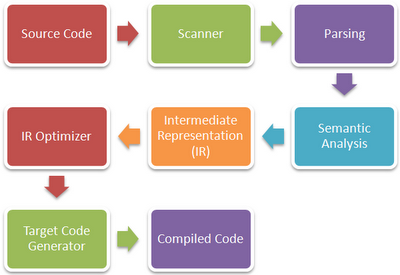
\includegraphics[width=\textwidth]{CompilerPhases} 
  \end{column}
  \end{columns}
\end{frame}
\begin{frame}{LLVM-IR}{How do I benefit ?}
\begin{columns}[T]

\begin{column}{0.5\textwidth}
\begin{itemize}
    \item Convert a language to LLVM-IR.
    \item Use either LLVM tools or your own.
    \item Sit back and let it work.
    \item You write the compiler only \alert{once}.
    \item Any platform that supports LLVM, Your code Also runs (analogy JAVA)
    \item With a few function calls, enable state-of-the-art JIT support. (NO coding)
    \item Free optimizations! (No coding)
\end{itemize}

\end{column}

\begin{column}{0.5\textwidth}
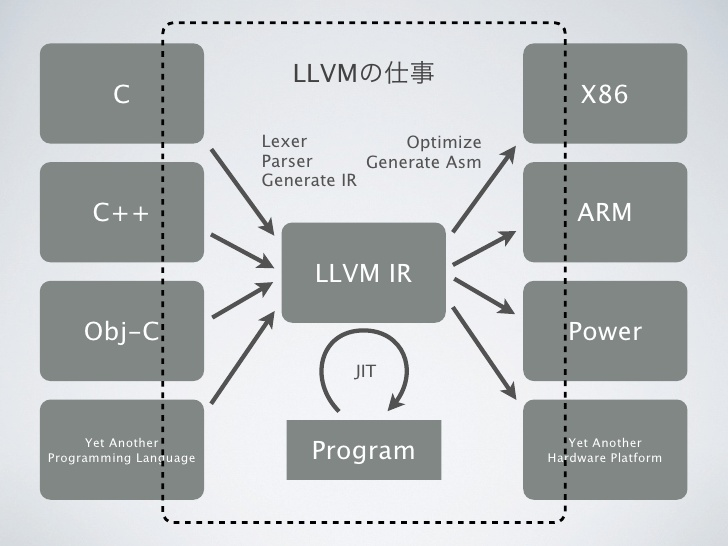
\includegraphics[width=\textwidth]{llvmir}\\
LLVM Pipeline\footnotemark
\footnotetext{Image Scraped from Internet}

\end{column}
\end{columns}  
\end{frame}
\begin{frame}{How does LLVM-IR look like ?}{Simple MIPS like assembly with infinite registers}
\begin{columns}

\begin{column}{0.5\textwidth}
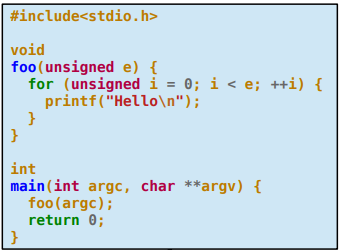
\includegraphics[scale=0.2,width=\textwidth]{code}

\end{column}

\begin{column}{0.5\textwidth}
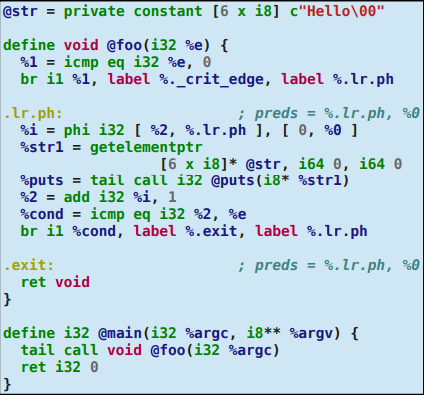
\includegraphics[scale=0.2, width=\textwidth]{ir}

\end{column}
\end{columns}
  
\end{frame}
\subsection{Background}

% You can reveal the parts of a slide one at a time
% with the \pause command:
\begin{frame}{Fork-Join Parallelism}{Intrinsic support from compilers}
  \begin{itemize}
  \item All mainstream compilers support fork-join parallelism.
  \item Provide support for Cilk Plus and OpenMP.
  \item Execution of Fork-Join creates a DAG.
  \item Execution usually via a \texttt{Work Stealing} Runtime.
\item Provide Serial Semantics.
  \end{itemize}
 \begin{block}{Serial Semantics}
That is, the result of a parallel run is the same as if the program had executed serially. Serial semantics makes it easier to reason about the parallel application.
\end{block} 
\end{frame}

\begin{frame}{Optimization :(}{Failure to optimize parallel code ![IR level]}
  \begin{columns}[T]
  \begin{column}{0.5\textwidth}
  \begin{itemize}
      \item Compilers can't optimize parallel code efficiently.
      \item Due to implementation of parallel constructs.
      \item They don't understand parallel constructs !
      \item All major compilers \alert{lower} parallel constructs to some primitives.
      \item No benefit from compiler optimizers. [IR level]
  \end{itemize}
  
  \end{column}
  \begin{column}{0.5\textwidth}
    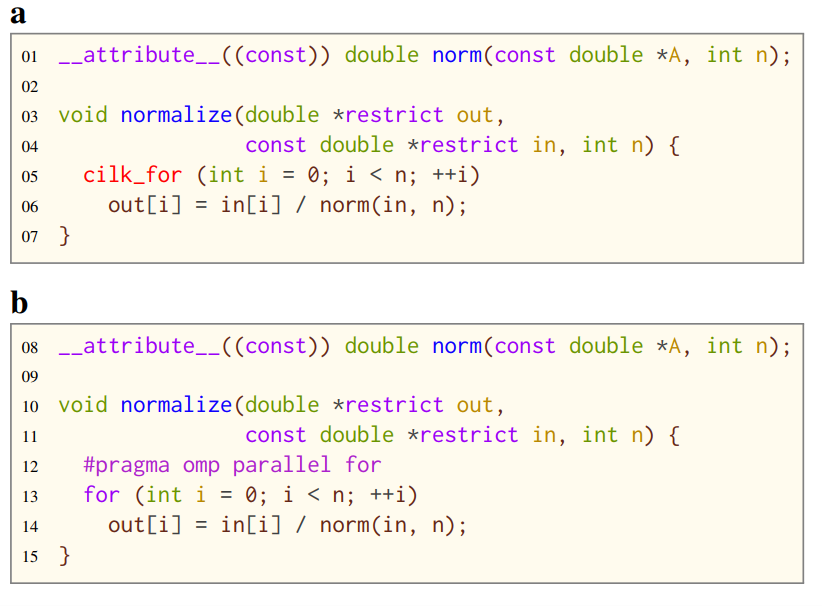
\includegraphics[scale=0.1, width=\textwidth]{opt_ex1}\\
    {\em a) Cilk Code  b) OpenMP Code}
  
  \end{column}
  
  \end{columns}
  
\end{frame}

\subsection{Motivation}
\begin{frame}{Parallel Encoding is Non Trivial}{Making IR aware of parallelism is hard !}
Use of serial code optimizers is dangerous for parallel programs.\\
It is not easy to encode Fork-Join parallelism in IR.\\
\begin{columns}[T]
  \begin{column}{0.5\textwidth}

  \begin{itemize}
      \item Using Meta-data for annotation
      \item Intrinsic functions to determine parallel tasks
      \item A brand new IR with native parallel support
      \item Modification of existing IR
  \end{itemize}
  \end{column}
  \begin{column}{0.5\textwidth}
  
\includegraphics[scale=0.2]{sad}
  \end{column}
\end{columns}
\end{frame}
\begin{frame}{Challenges}{Why can't we re-implement an new IR}

\begin{itemize}
    \item Introducing a new IR only work in academia, not Industry.
    \item Even if implemented, it would be painful, as it has complex dependencies.
    \item All previous approaches exhibited problems with serial optimizers.
    \item Elaborate Intrusive changes to existing compiler codebase is needed.
\end{itemize}
  
\end{frame}

\section{Main Paper}


\subsection{Contribution}
\begin{frame}{TAPIR Contribution}{Annotate existing IR with minimum changes}
\begin{columns}[T]
  \begin{column}{0.7\textwidth}
\begin{itemize}
    \item Parallel aware IR represents fork-join parallelism asymmetrically, enabling serial \& parallel optimizations.
    \item A mere 6000 lines addition to 4 Million lines of LLVM (0.15\%)
    \item Implementation of parallel loop scheduling \& elimination of unnecessary sync.
    \item Experiments and a reference implementation for benchmarks.
\end{itemize}
\end{column}
  \begin{column}{0.3\textwidth}
  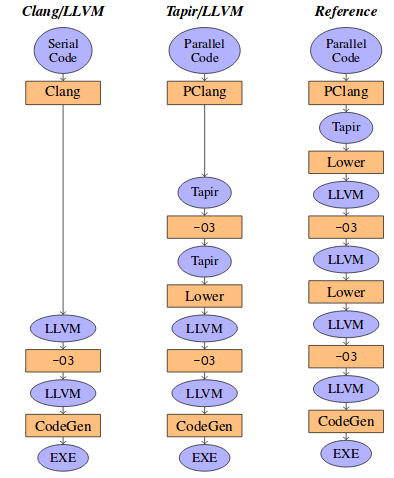
\includegraphics[scale=.25]{llvm}
  \end{column}
\end{columns} 
\end{frame}

\subsection{Related Work}
\begin{frame}{Related Work}
    \begin{itemize}
    \item Finding and Removing Unnecessary synchronization in Java.\footnote{ref [3]}
    \item Detection of instructions unaffected by parallel threads.\footnote{ref [26]}
    \item  Modification of  LLVM  IR  to  support  Open-SHMEM.\footnote{ref [30]}
    \item  Inter-procedural  analysis  to  perform various optimizations in critical Section Code \footnote{ref [6, 7]}
    \end{itemize}
    
\end{frame}
\subsection{Implementation}
\begin{frame}{Implementation I}
    \begin{itemize}
        \item Addition of 3 instructions to IR:
        \begin{itemize}
            \item detach (\texttt{async})
            \item reattach (\texttt{join})
            \item sync      (\texttt{barrier})
        \end{itemize}
        \item Minor differences with what we have seen.
        \item Advantages:
        \begin{itemize}
            \item Easy introduction of Fork-Join in Compilers
            \item Expressive IR to encode Fork-Join of different Languages.
            \item Plays nicely with serial optimizers.
            \item Performance gains in practical scenarios.
        \end{itemize}
    \end{itemize}
\end{frame}
\begin{frame}{Implementation II}
\begin{columns}
\begin{column}{0.7\textwidth}
\begin{itemize}
    \item The SSA form for LLVM IR must be adapted for Tapir.
    \item detach/reattach express parallel tasks asymmetrically  both  syntactically and semantically as in memory.
    \item Optimizations
    \begin{itemize}
        \item Common sub-expression elimination
        \item Loop-Invariant code Motion
        \item TRE (recursion elimination)
        \item Loop Scheduling.
        \item .... many more
    \end{itemize}
    
    \end{itemize}
    \end{column}
    \begin{column}{0.3\textwidth}
    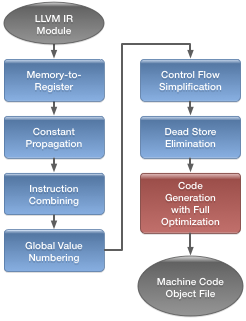
\includegraphics[width=\textwidth]{optp}
    \end{column}
    \end{columns}
    
\end{frame}

\subsection{Result}
\begin{frame}{Result}

\centering 
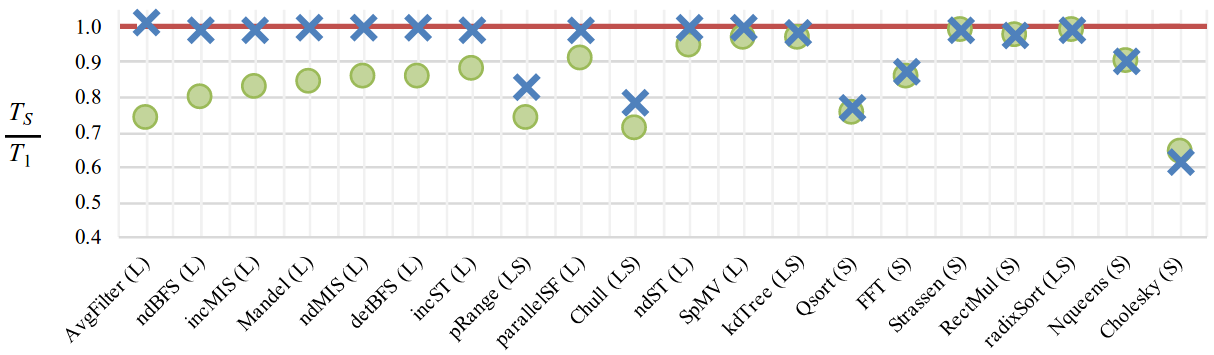
\includegraphics[width=\textwidth]{result}
{ \em O: reference compiler $|$  X: tapir/llvm }


\end{frame}

\subsection{Conclusion}

\begin{frame}{Conclusion}
\begin{itemize}
    \item TAPIR makes it very easy to write \alert{Optimization Passes}.\footnote{http://llvm.org/docs/Passes.html}
    \item Tapir enables FJP programs to benefit from both serial and parallel optimizations.
    \item  Serial programs work on parallel constructs with little or no modification.
\end{itemize}
\end{frame}


\section*{Questions}

\begin{frame}{Questions}{Interested people can opt for Advanced Compiler Optimization (Next Sem)}
\centering

\includegraphics[scale=1]{questions}
\end{frame}



% All of the following is optional and typically not needed. 
\appendix
\section<presentation>*{\appendixname}
\subsection<presentation>*{For Further Reading}

\begin{frame}[allowframebreaks]
  \frametitle<presentation>{For Further Reading}
    
  \begin{thebibliography}{10}
    
  \beamertemplatebookbibitems
  % Start with overview books.

  \bibitem{Aho}
    A.~V~.~Aho
    \newblock {\em Compilers:
Principles, Techniques, and Tools}.
    \newblock Addison-Wesley, 2006.
 
    
  \beamertemplatearticlebibitems
  % Followed by interesting articles. Keep the list short. 

  \bibitem{LLVM}
    LLVM Website.
    \newblock{\em www.llvm.org}
  \end{thebibliography}
\end{frame}

\end{document}
